An \define{environment diagram} keeps track of all the variables that have been
defined and the values they are bound to. We will be using this tool throughout
the course to understand complex programs involving several different objects
and function calls.

\begin{minipage}{0.3\linewidth}
\begin{lstlisting}[linewidth=\linewidth]
x = 3

def square(x):
    return x ** 2

square(2)
\end{lstlisting}
\end{minipage}%
\begin{minipage}{0.7\linewidth}
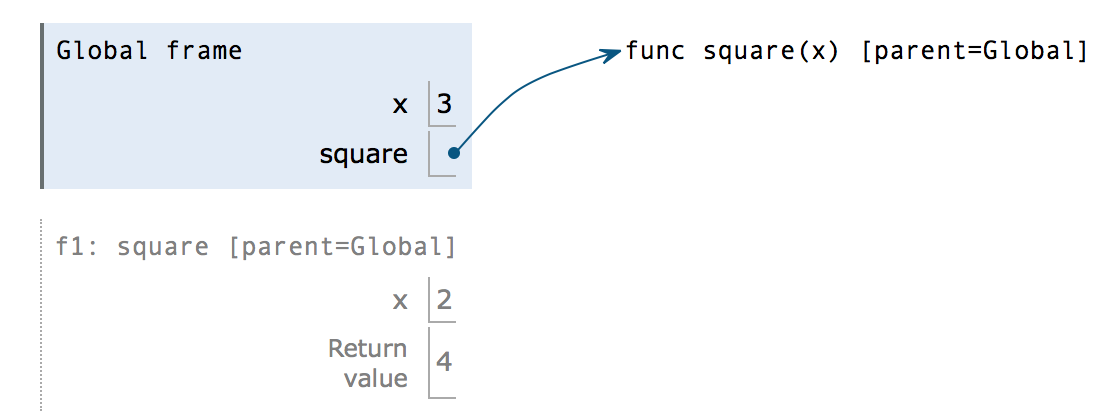
\includegraphics[width=\linewidth]{simpler_hof.png}
\end{minipage}

Remember that programs are simply a set of statements, or instructions, so
drawing diagrams that represent these programs also involve following sets
of instructions! Let's dive in. \\\\

\subsection*{Assignment Statements}
\emph{Assignment statements}, such as \texttt{x = 3}, define variables in
programs. To execute one in an environment diagram, record the variable name
and the value:

\begin{enumerate}
    \item Evaluate the expression on the right side of the \texttt{=} sign
    \item Write the variable name and the expression's value in the current
    frame. \\
\end{enumerate}

\begin{questions}
\subimport{../../../topics/functions-and-expressions/code/env-diagrams/}{assignment-statements.tex}

\newpage

\subsection*{\text{def} Statements}
\emph{\texttt{def} statements} create function objects and bind them to a name.
To diagram \texttt{def} statements, record the function name and bind the
function object to the name. It's also important to write the \define{parent
frame} of the function, which is where the function is defined.

\begin{enumerate}
    \item Draw the function object to the right-hand-side of the frames,
    denoting the intrinsic name of the function, its parameters, and the parent
    frame (e.g. \texttt{func square(x) [parent = Global]}.
        \footnote{When importing functions, we still create a function object in the environment
        diagram, bound to the name of the imported function. However, the parent and parameters
        of an imported function is unknown so only the function's name is included.
        For example, if we imported the function \texttt{add}, the function object would just be
        \texttt{add(...)}}
    \item Write the function name in the current frame and draw an arrow from the
    name to the function object. \\
\end{enumerate}

\subimport{../../../topics/functions-and-expressions/code/env-diagrams/}{def-statements.tex}

\newpage

\subsection*{Call Expressions}
\emph{Call expressions}, such as \texttt{square(2)}, apply functions to
arguments. When executing call expressions, we create a new frame in our
diagram to keep track of local variables:

\setlength{\skip\footins}{3 in}
\begin{enumerate}
    \item Evaluate the operator, which should evaluate to a function.
    \item Evaluate the operands from left to right.
    \item Draw a new frame, labelling it with the following:
        \footnote{Since we do not know how built-in functions
            like \texttt{min(...)} or imported functions like \texttt{add(...)} are implemented,
            we do \emph{not} draw a new frame when we call them.}
        \begin{itemize}
            \item A unique index (\texttt{f1}, \texttt{f2}, \texttt{f3}, ...)
            \item The \define{intrinsic name} of the function, which is the
            name of the function object itself. For example, if the function
            object is \texttt{func square(x) [parent=Global]}, the intrinsic
            name is \texttt{square}.
            \item The parent frame (\texttt{[parent=Global]})
        \end{itemize}
    \item Bind the formal parameters to the argument values obtained in step 2
    (e.g.\ bind \texttt{x} to 3).
    \item Evaluate the body of the function in this new frame until a return
    value is obtained. Write down the return value in the frame.
\end{enumerate}

If a function does not have a return value, it implicitly returns
\texttt{None}.  In that case, the ``Return value'' box should contain
\texttt{None}. \\

\subimport{../../../topics/functions-and-expressions/code/env-diagrams/}{call-expressions.tex}

\subimport{../../../topics/functions-and-expressions/medium/env-diagram/}{xfg.tex}
\end{questions}

